\section{Preliminary Results}

%--------------------------------------------------------

\begin{frame}
\frametitle{Preliminary Results}

\centering
\scriptsize
ALICE Pb--Pb $\sqrt{s_{NN}}=2.76$ TeV

HEPData: \texttt{ins1222333}

\vspace{0.15cm}

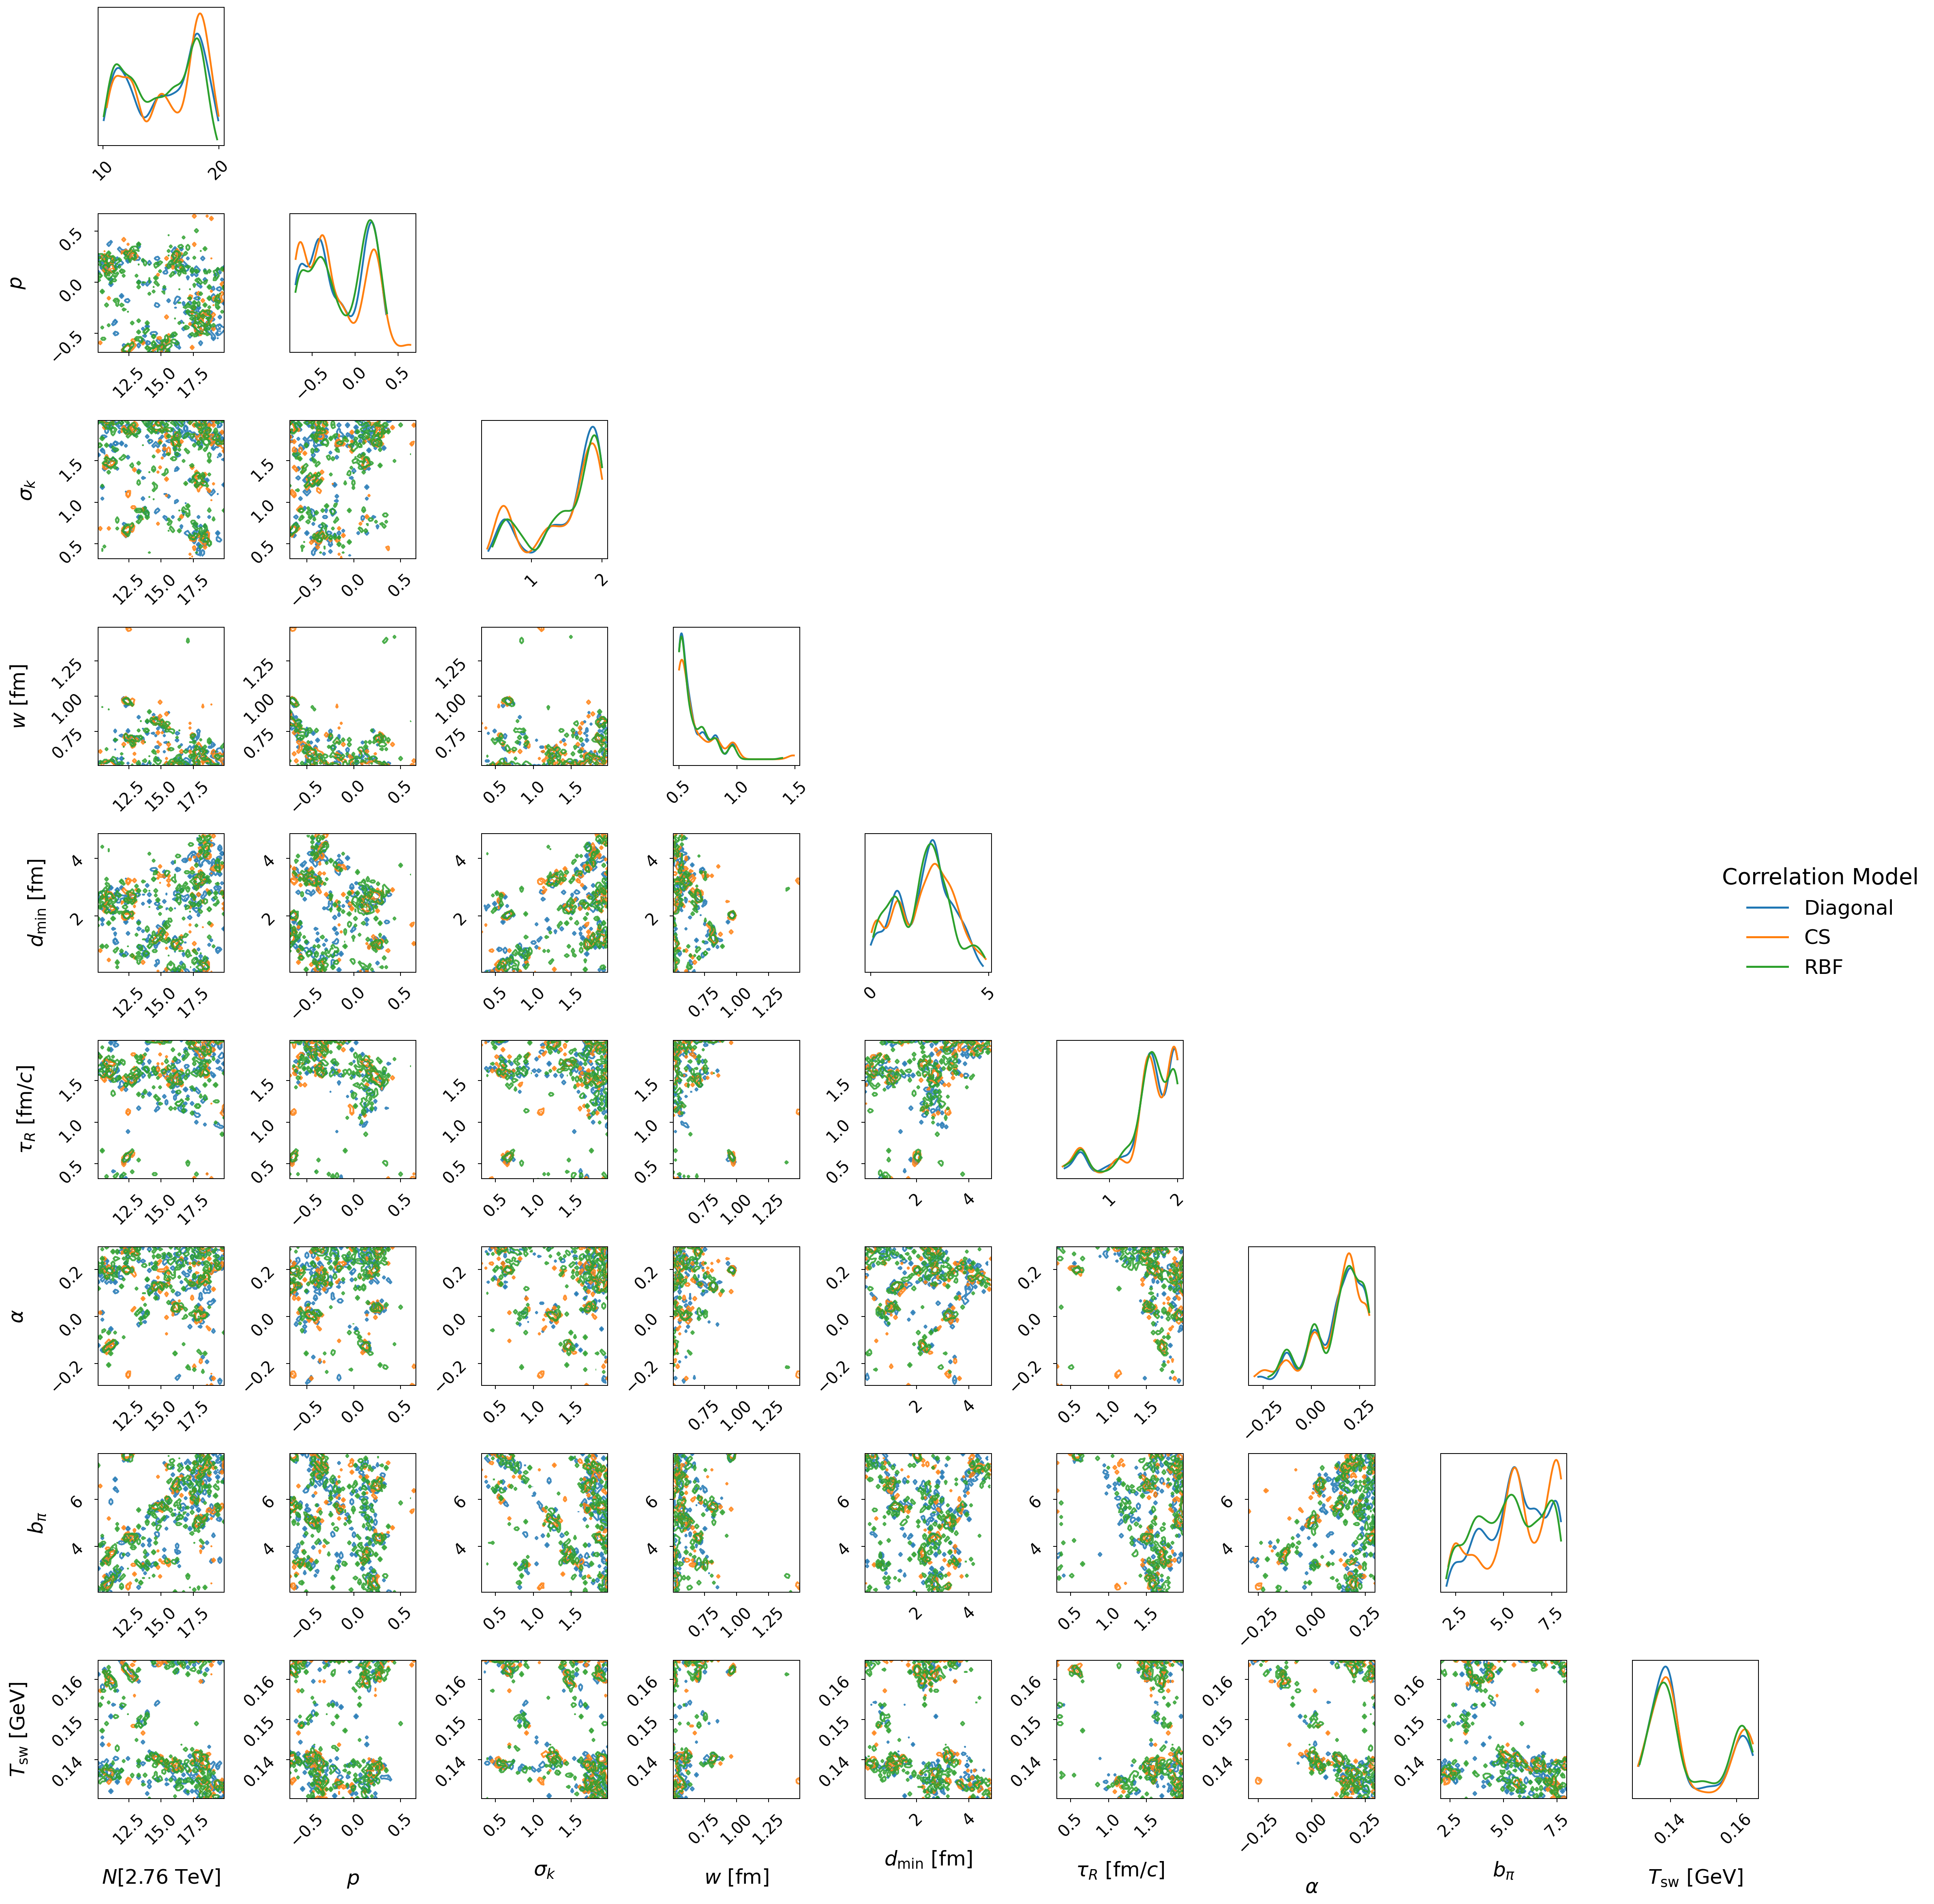
\includegraphics[width=0.48\textwidth]{img/corner_all_models_1.png}
\hfill
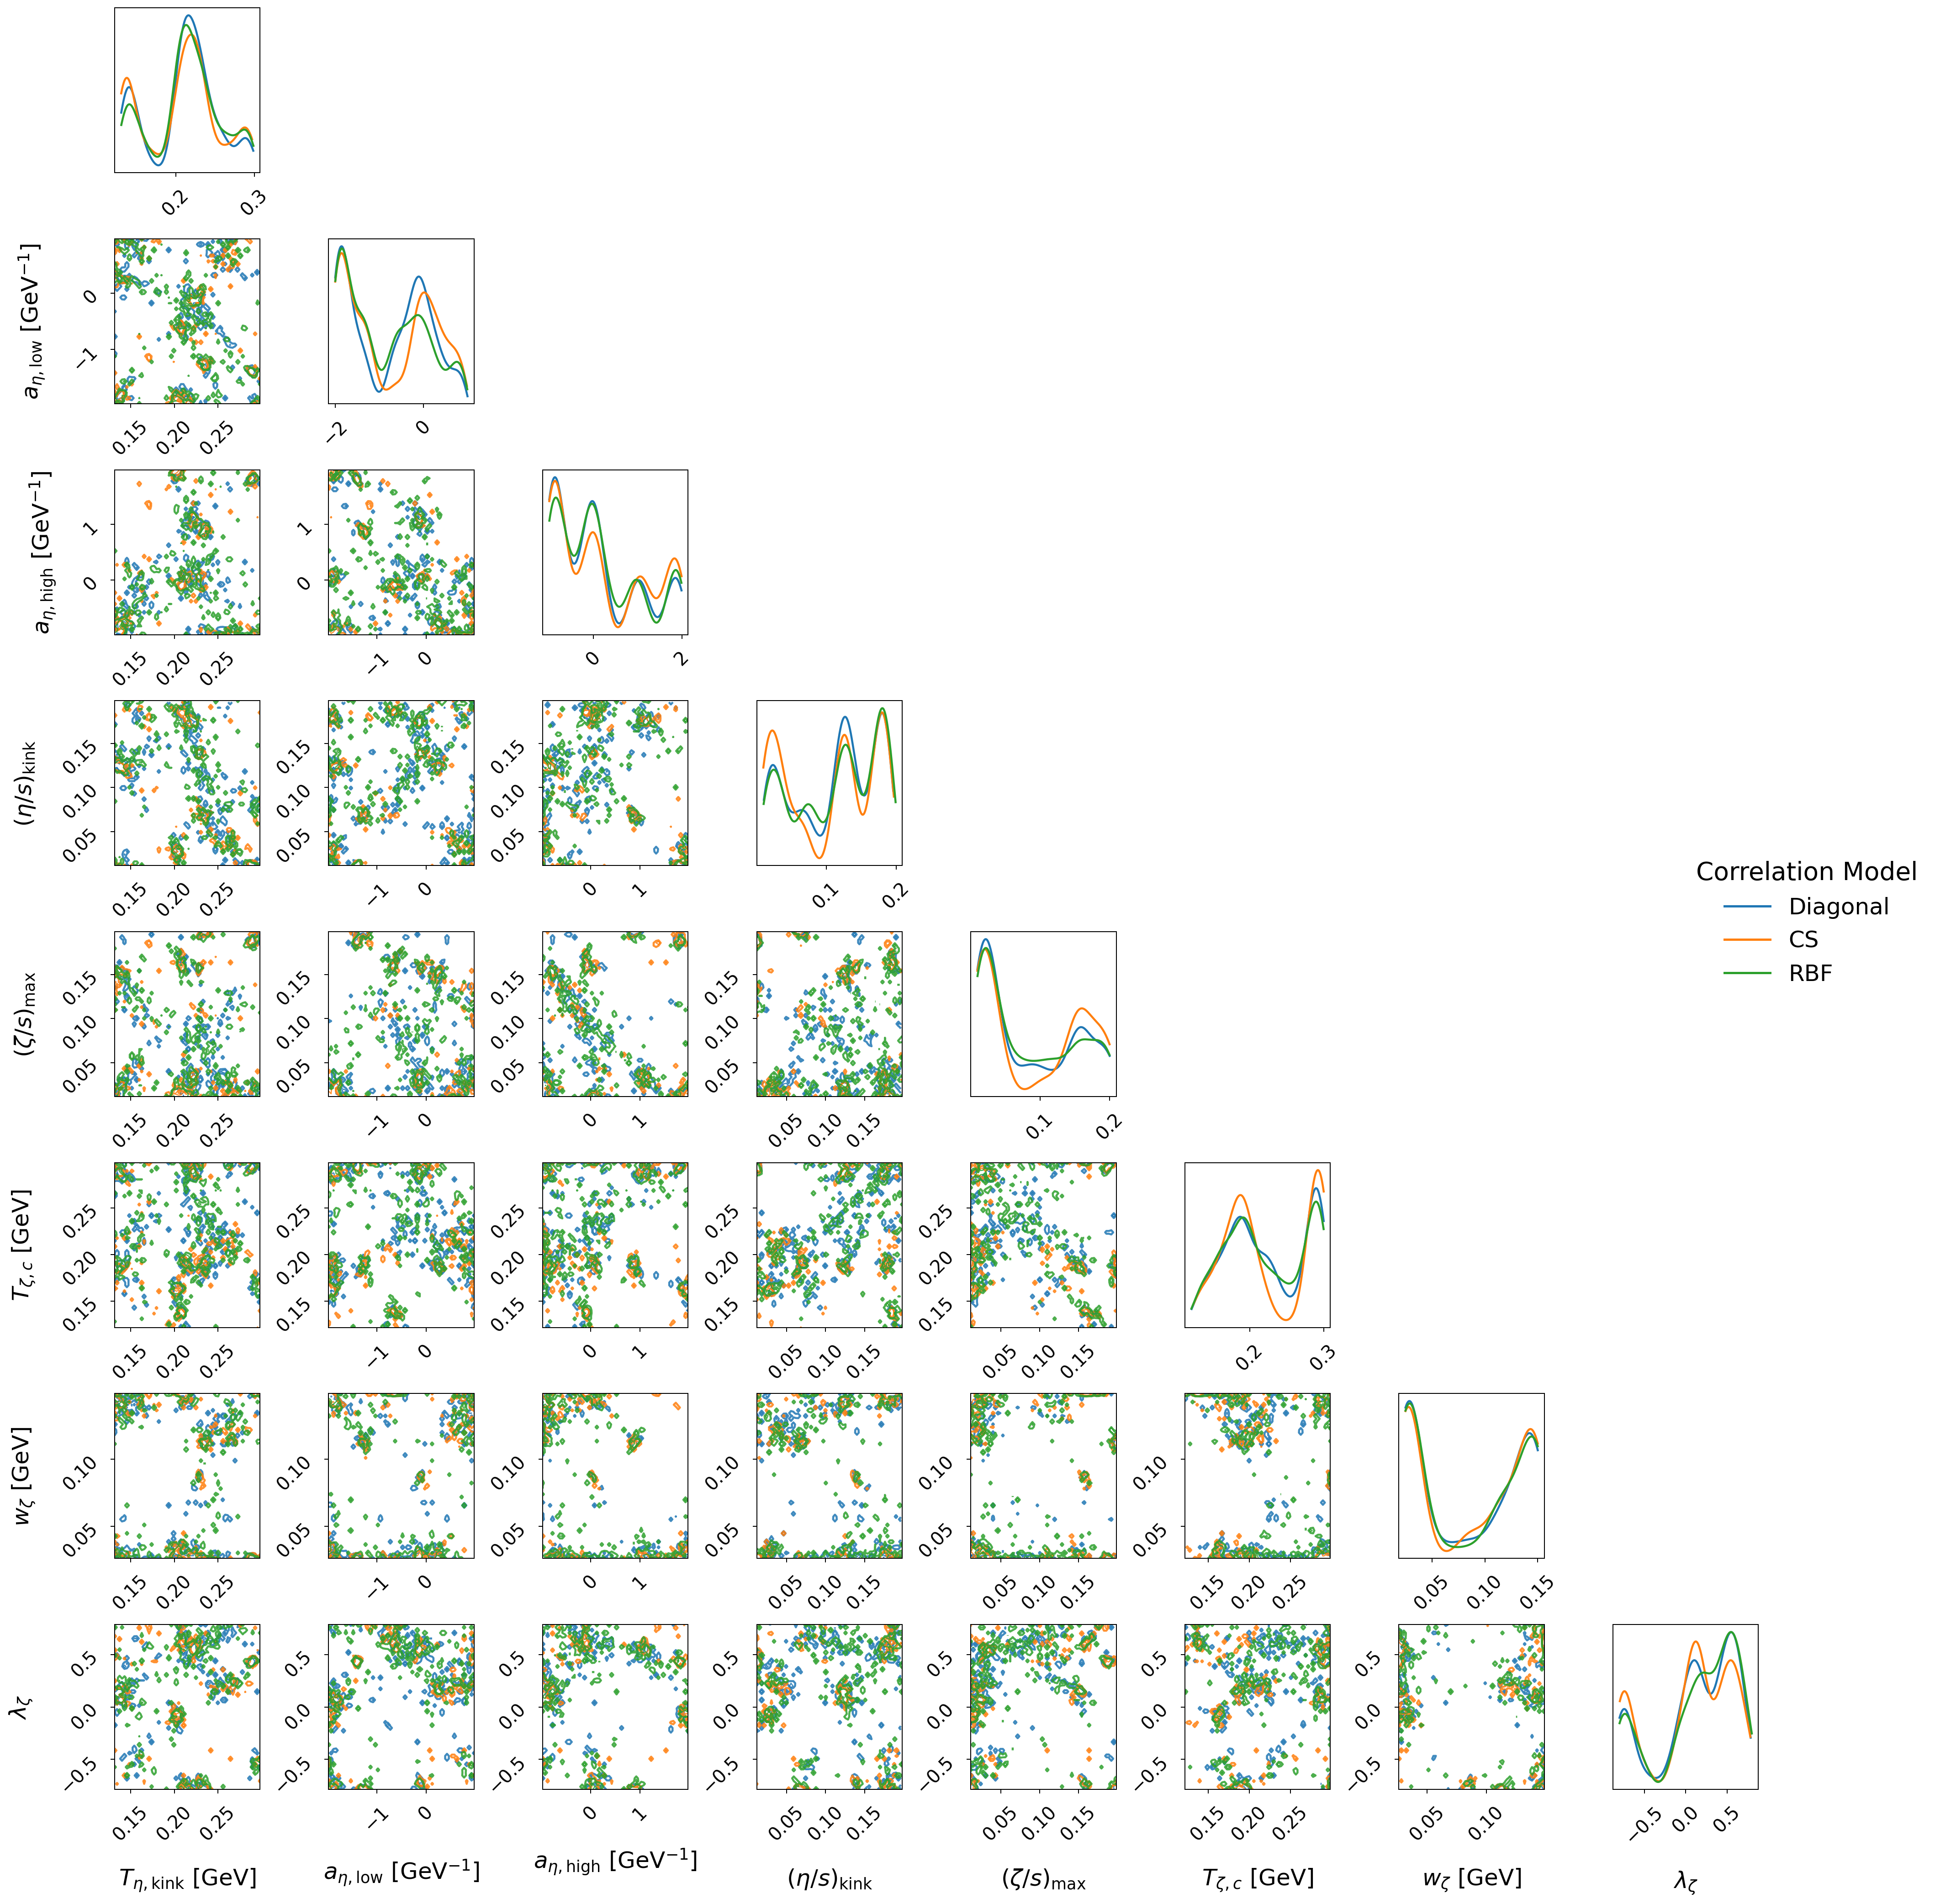
\includegraphics[width=0.48\textwidth]{img/corner_all_models_2.png}


\tiny
Posterior distributions using diagonal, compound-symmetry (CS), and RBF covariance models.

\end{frame}

%--------------------------------------------------------

% \begin{frame}
% \frametitle{Transport Parameter Constraints}

% \centering
% \scriptsize
% ALICE Pb--Pb $\sqrt{s_{NN}}=2.76$ TeV

% HEPData: \texttt{ins1222333}

% \vspace{0.15cm}

% 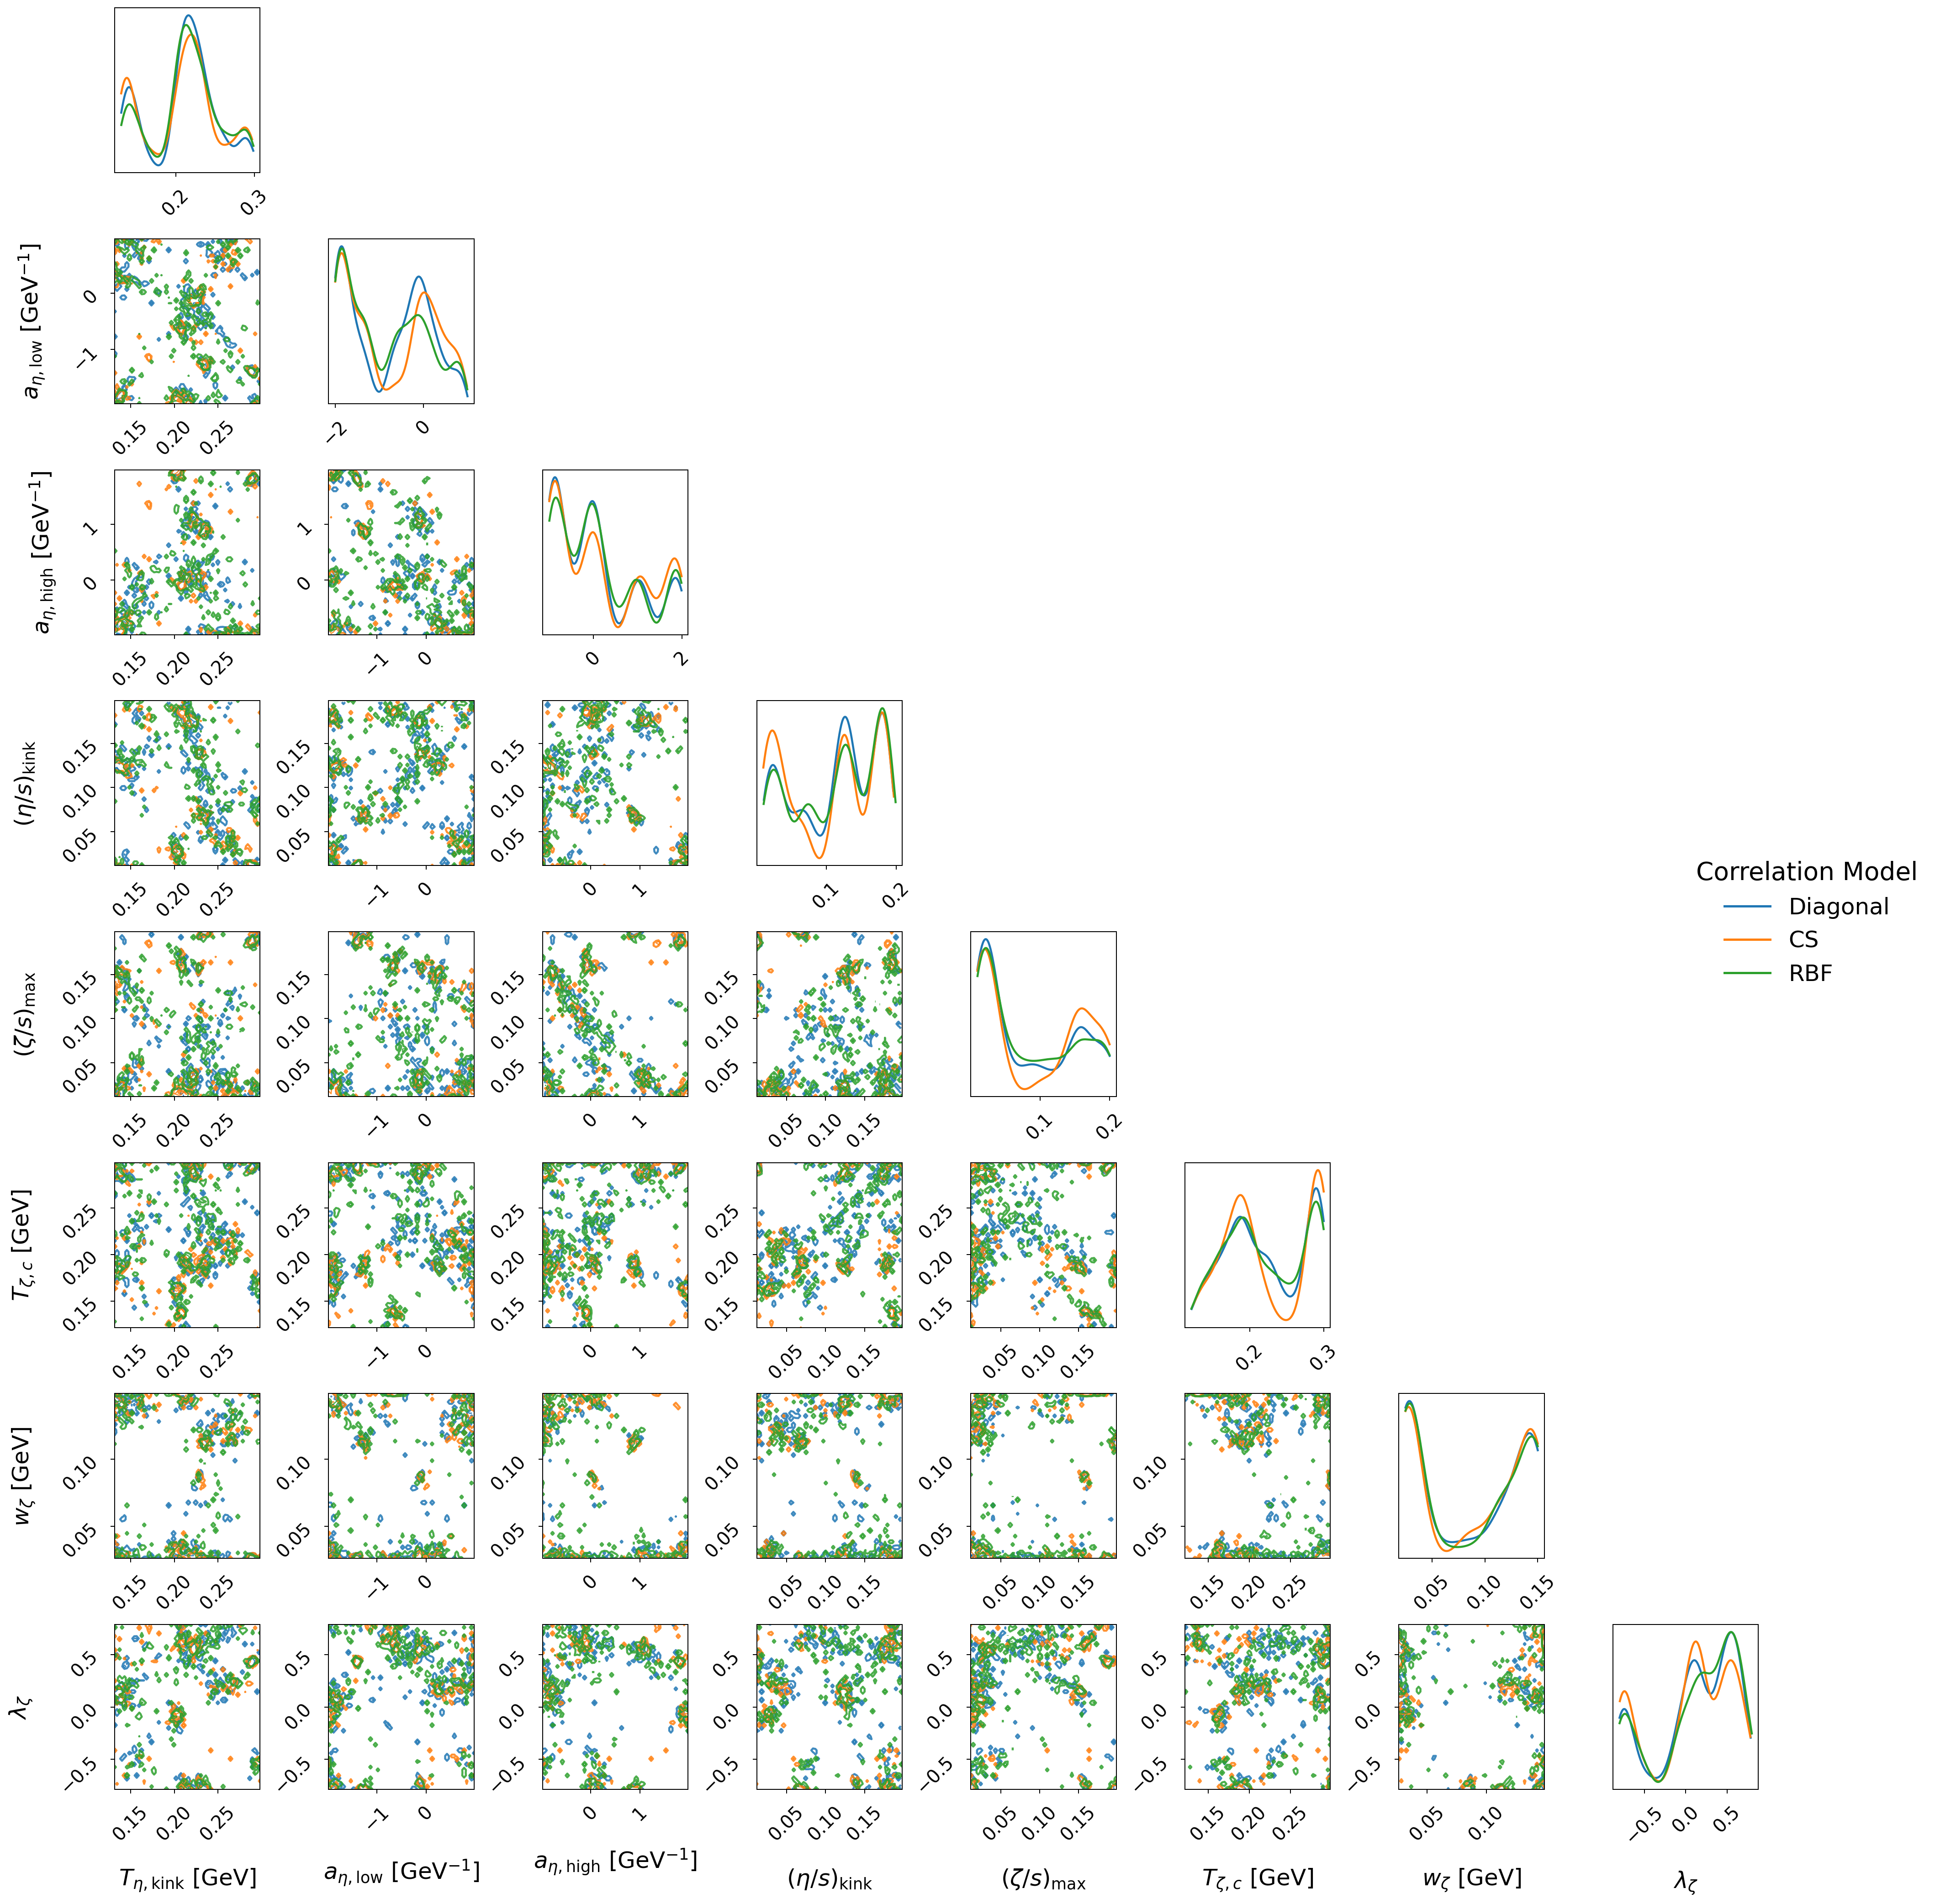
\includegraphics[width=0.48\textwidth]{img/corner_all_models_2.png}
% \hfill
% 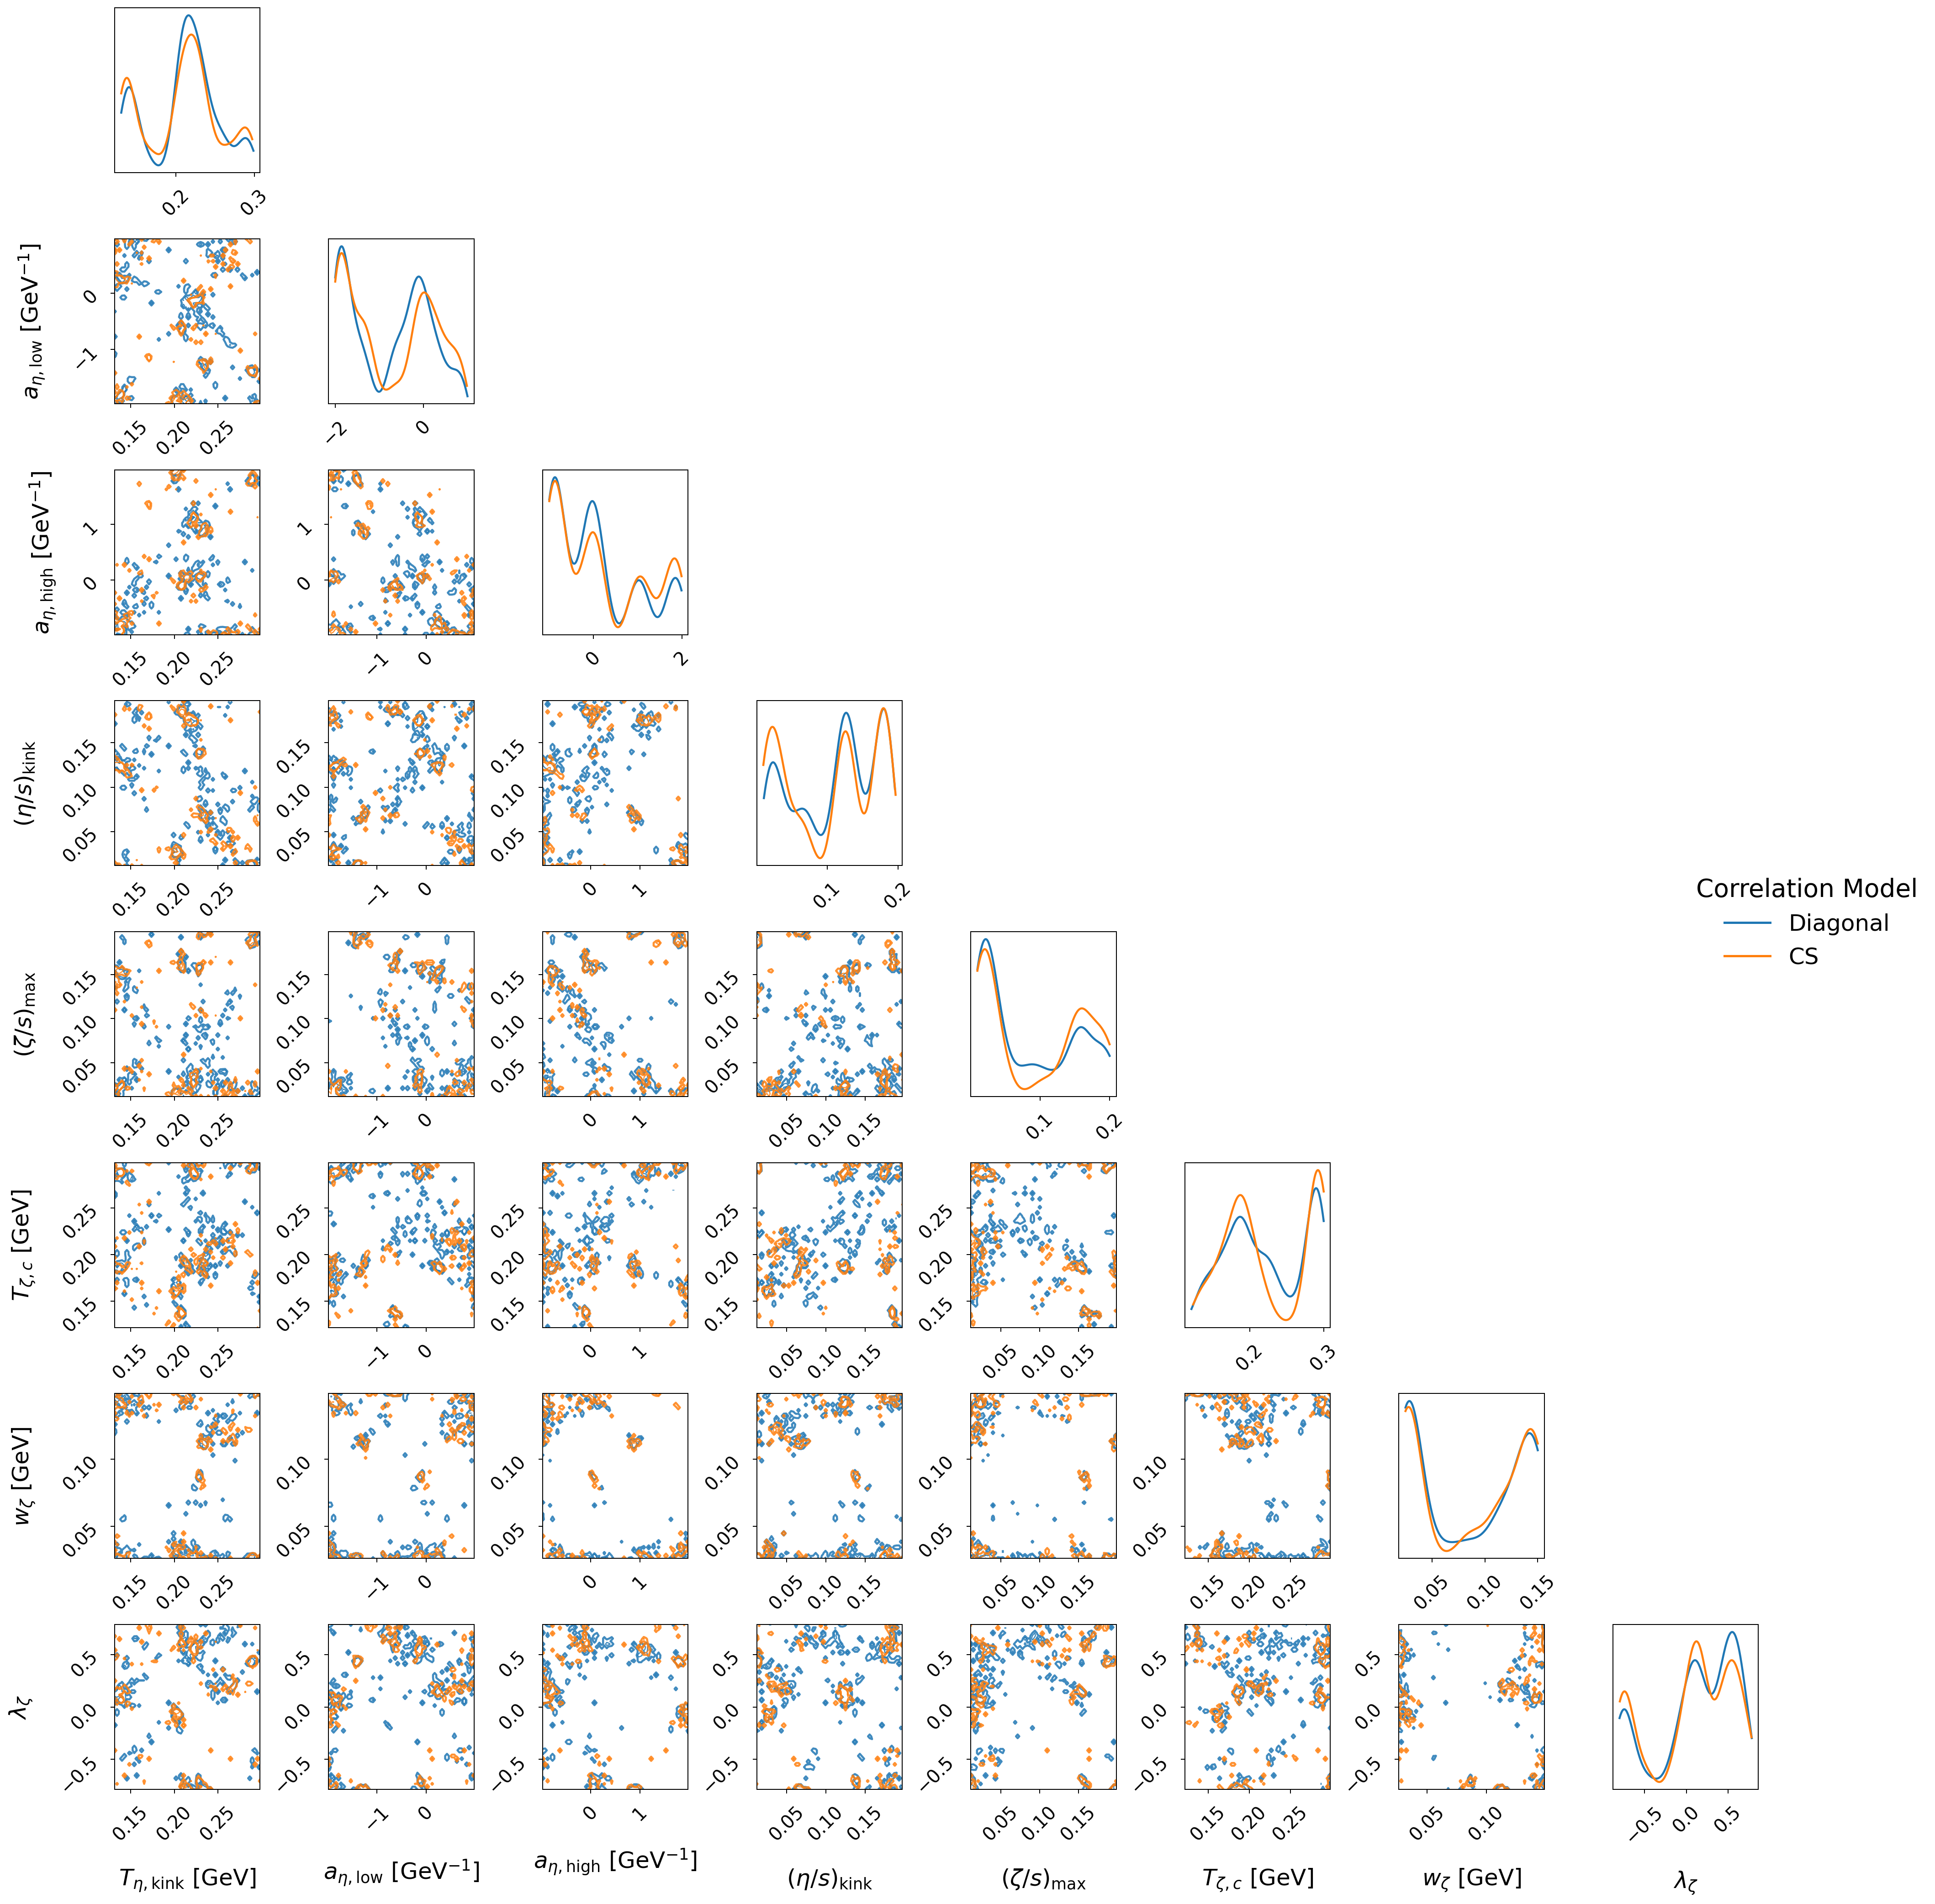
\includegraphics[width=0.48\textwidth]{img/corner_diag_vs_cs_2.png}

% \vspace{0.15cm}

% \tiny
% Left: posterior distributions using diagonal, compound-symmetry (CS), and RBF covariance models.
% Right: comparison between the diagonal and CS covariance models.

% \end{frame}

% %--------------------------------------------------------

% \begin{frame}
% \frametitle{Diagonal vs RBF: Initial-State Parameters}

% \centering
% \scriptsize
% ALICE Pb--Pb $\sqrt{s_{NN}}=2.76$ TeV

% HEPData: \texttt{ins1222333}

% \vspace{0.15cm}

% 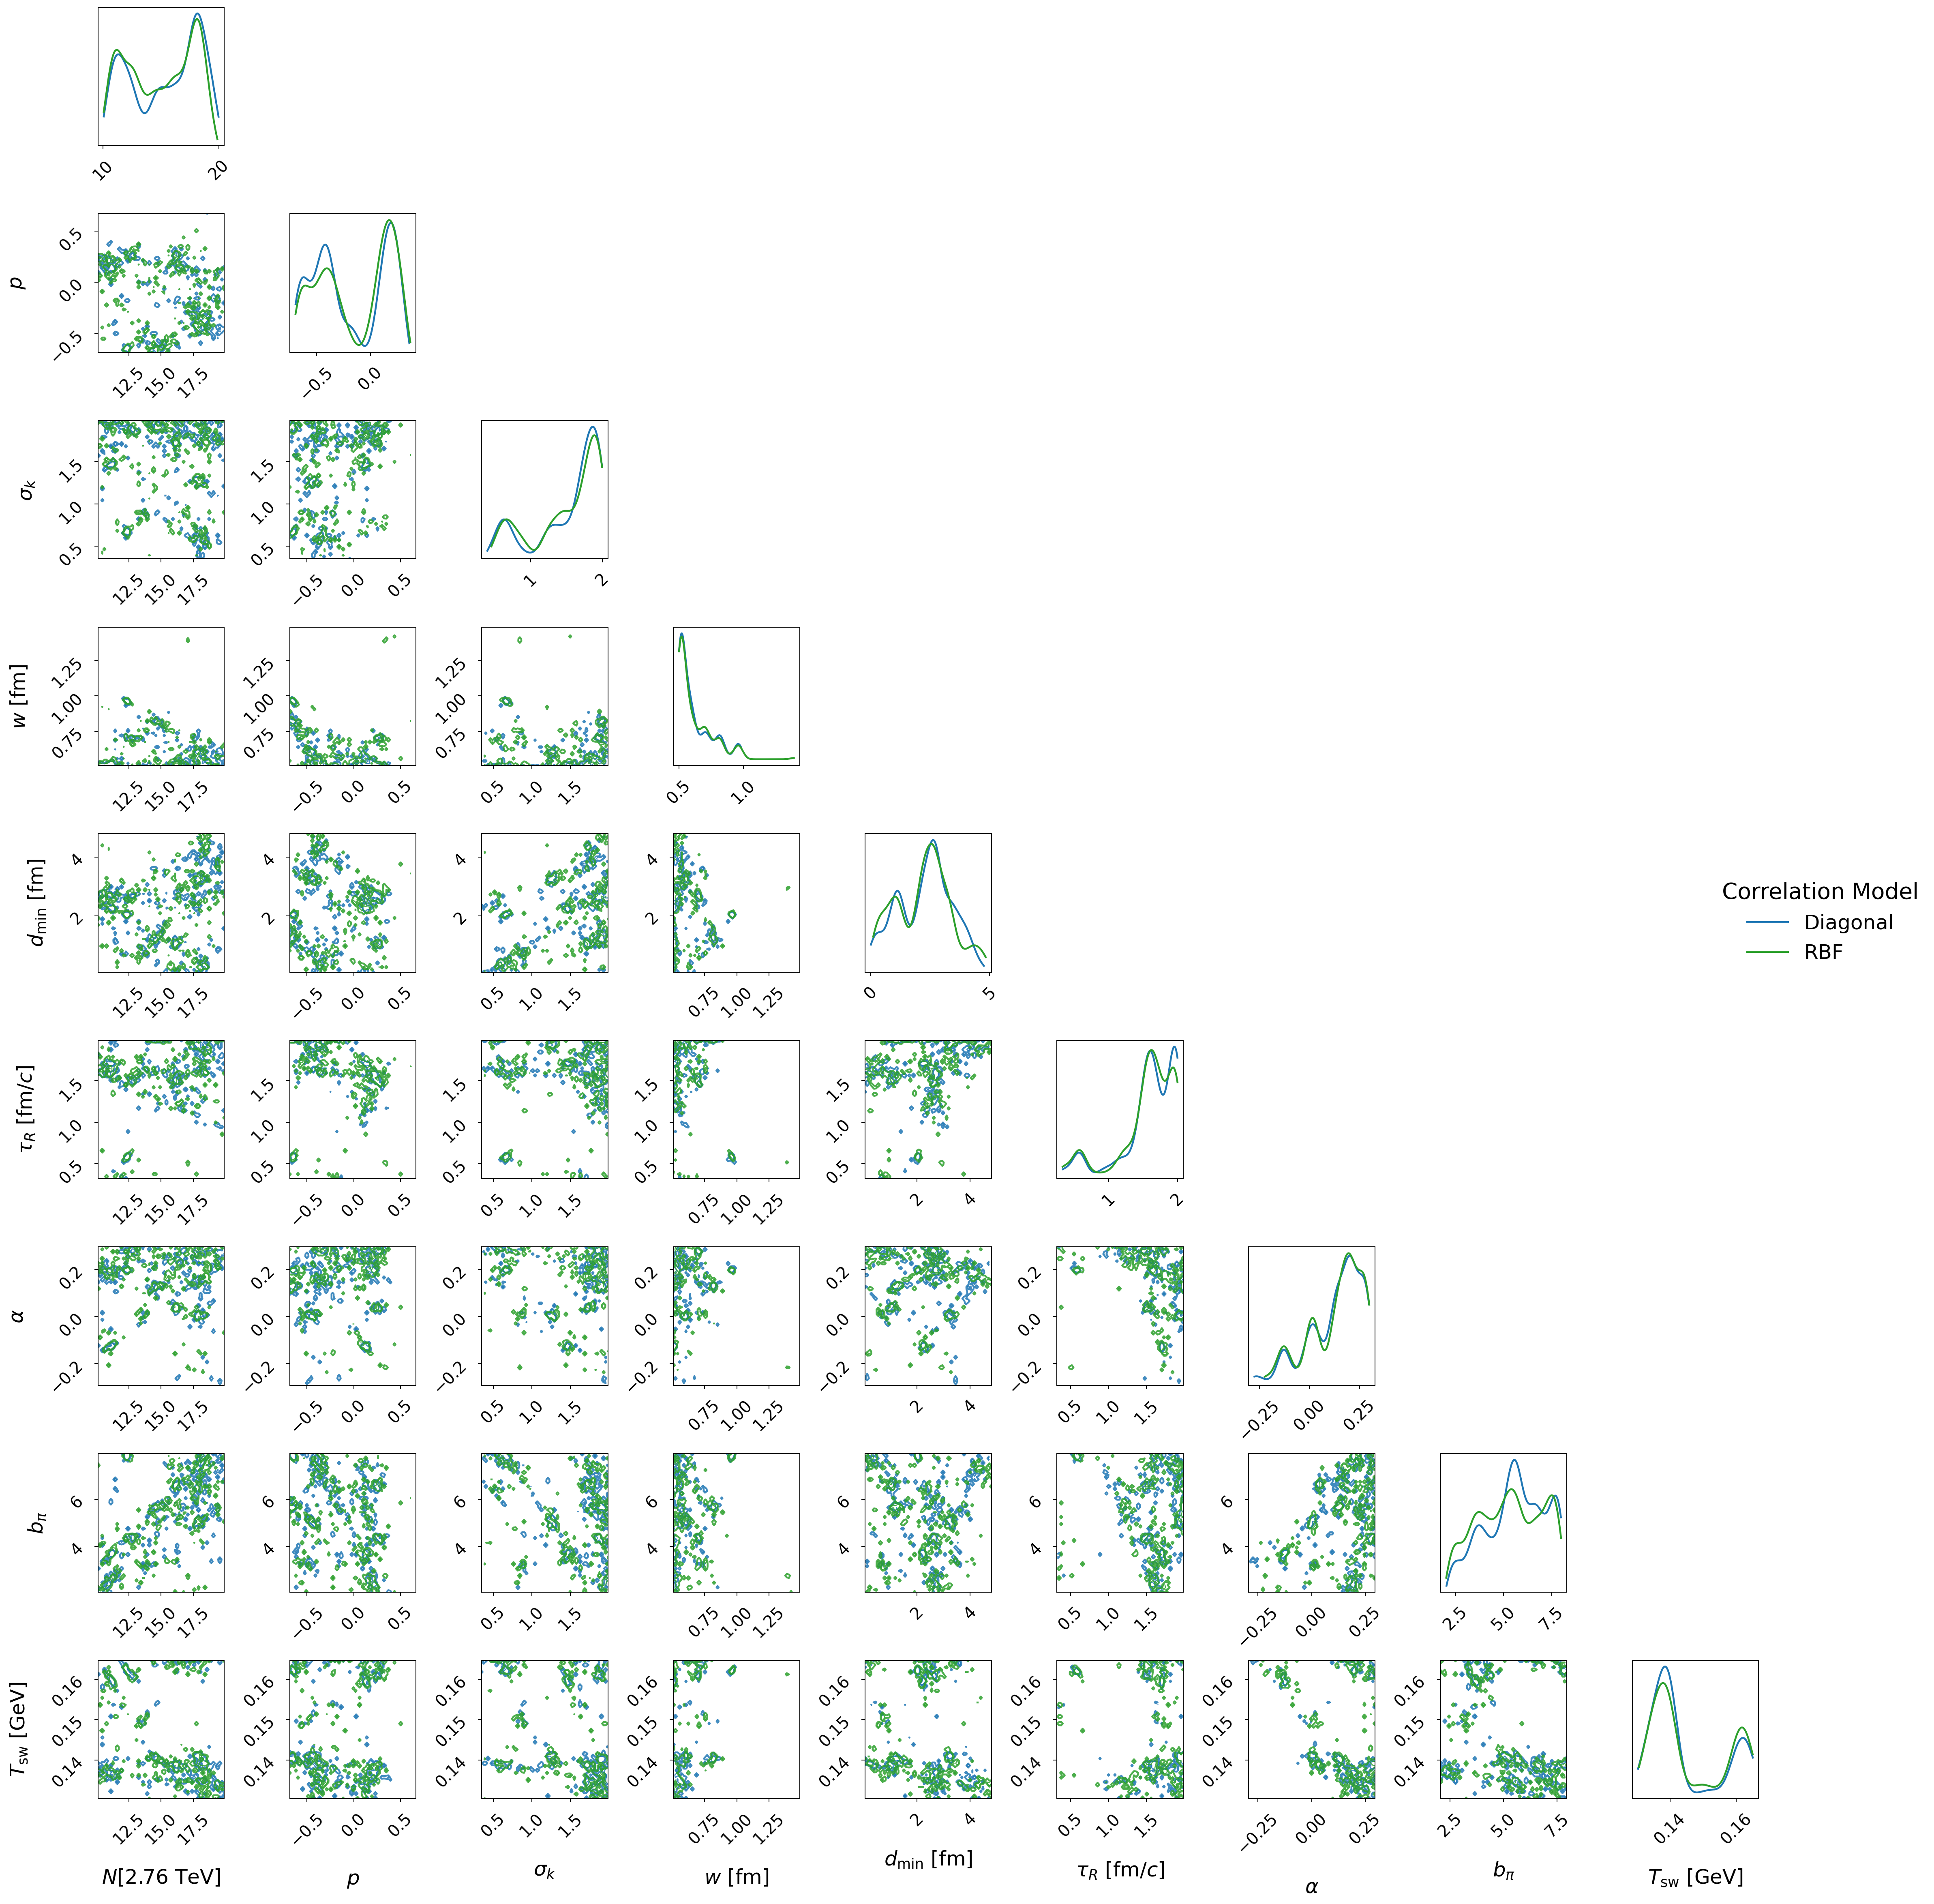
\includegraphics[width=0.82\textwidth]{img/corner_diag_vs_rbf_1.png}

% \vspace{0.15cm}

% \tiny
% Comparison between the diagonal and RBF experimental covariance models.

% \end{frame}

% %--------------------------------------------------------

% \begin{frame}
% \frametitle{Diagonal vs RBF: Transport Parameters}

% \centering
% \scriptsize
% ALICE Pb--Pb $\sqrt{s_{NN}}=2.76$ TeV

% HEPData: \texttt{ins1222333}

% \vspace{0.15cm}

% 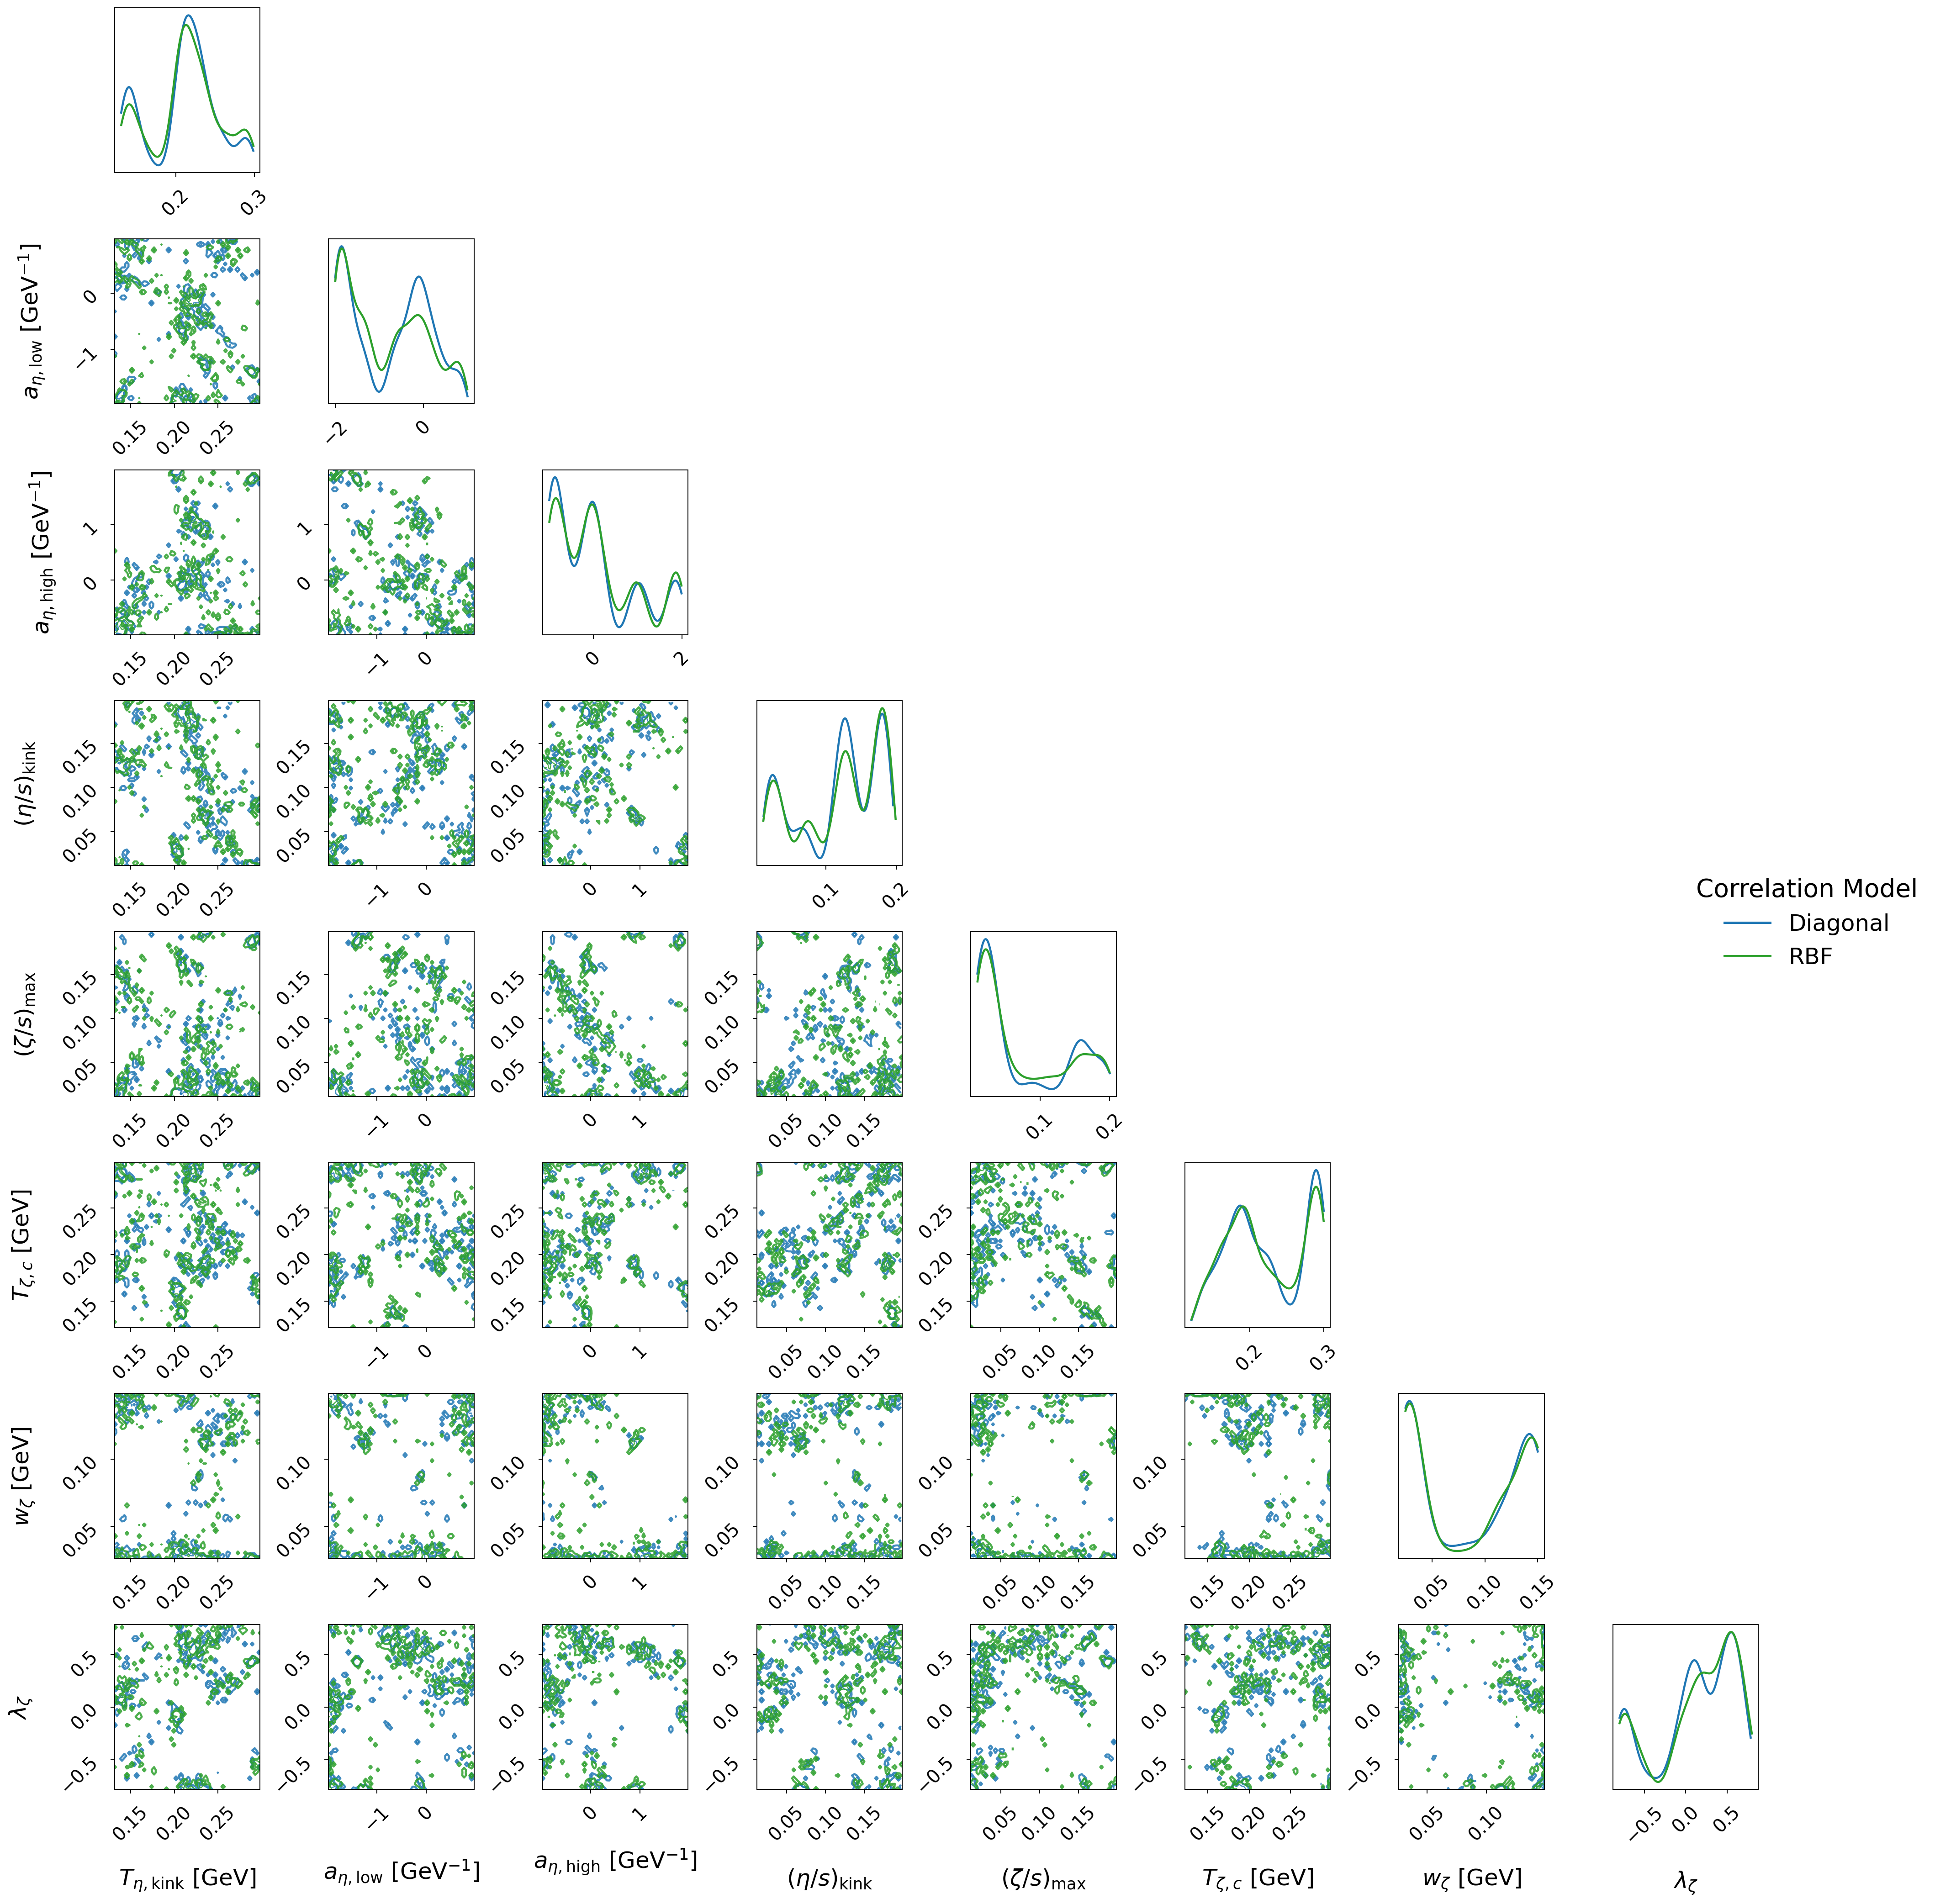
\includegraphics[width=0.82\textwidth]{img/corner_diag_vs_rbf_2.png}

% \vspace{0.15cm}

% \tiny
% Comparison between the diagonal and RBF experimental covariance models.

% \end{frame}